\RequirePackage[abort, l2tabu, orthodox]{nag}
\documentclass[pageno]{jpaper}

% standard LaTeX packages that do not interfere with hyperref
\usepackage{alltt}
\usepackage{amssymb}
\usepackage{booktabs}
\usepackage{caption}
\usepackage[draft]{fixme}
\usepackage{epstopdf}
\usepackage{flushend}
\usepackage{graphicx}
\usepackage[final]{listings}
\usepackage[sort&compress]{natbib}
\usepackage{tikz}
\usepackage[normalem]{ulem}
\usepackage{xspace}
\usepackage{rotating}
\usepackage{adjustbox}
\usepackage{balance}

% font selection
\usepackage{courier}
\usepackage{helvet}
\usepackage{mathptmx}
\usepackage{microtype}
\usepackage[mathscr]{euscript}

% hyperref itself
\usepackage{hyperref}

% standard packages that must be loaded after hyperref
\usepackage{bookmark}
\usepackage{verbatim}

% should be loaded after listings and subfig
\usepackage{cleveref}
\usepackage{multirow}
\usepackage{xfrac}

% custom packages for this paper
\usepackage{xcolor}
\usepackage{amsmath}

%\DeclareCaptionType{copyrightbox}

\renewcommand{\cite}[1]{%
  \PackageError{natbib}{%
    The \string\cite\space{} command is ambiguous; use
    \string\citet\space{} or \string\citep\space{} instead}{}}

\renewcommand{\autoref}[1]{%
  \PackageError{cleveref}{%
    Do not use \string\autoref.  Use \string\cref instead, or use
    \string\crefrange for ranges of referenced items}}

\renewcommand{\hline}[1]{%
  \PackageError{booktabs}{%
    Do not use \string\hline.  Use \string\toprule, \string\midrule,
    or \string\bottomrule\space instead depending on where in the
    table the line appears}}

\newcommand{\email}[1]{\href{mailto:#1@cs.cmu.edu}{#1}}

% cleveref configuration
\crefname{figure}{Figure}{Figures}
\crefname{section}{Section}{Sections}
\crefname{table}{Table}{Tables}

\hyphenation{test-case}

% lst configuration
\lstdefinelanguage{example}{%
  morekeywords={xyz},
}

\lstset{
  basicstyle=\sffamily,
  columns=fullflexible,
  numbersep=5pt,
  numberstyle=\scriptsize,
  showstringspaces=false,
  language=example,
  escapeinside={/*@}{@*/},
  belowcaptionskip=1\baselineskip,
  language=C,
  showstringspaces=false,
  keywordstyle=\bfseries,
  commentstyle=\itshape,
}


\urlstyle{sf}

\pdfpagewidth=8.5in
\pdfpageheight=11in


% Custom commands
\newcommand{\Tool}{\textsc{XYZ}\xspace}

%\sloppy
% start doc
\begin{document}

\title{
  \textsc{\LARGE Final Report\\
  \Large Automatic Tuning of DBMS using Machine Learning\\
  \large CMU 10-701: Machine Learning (Fall 2014)}
}

\author{Joy Arulraj \hspace{0.1 in} Ram Raghunathan \hspace{0.1 in} \\
{\{\email{jarulraj}, \email{rraghuna}\}}}

\date{}
\maketitle


\begin{abstract} 
Hardware support for transactional memory in the form of
transaction synchronization instruction set extensions has been introduced in
recent Intel processors \citep{tsx-intro}. These extensions provide two software
interfaces to define transaction regions: a flexible interface which allows the programmer
to specify a fallback path to handle transaction failures (Restricted
Transactional Memory) and another backward compatible interface that is less
customisable (Hardware Lock Elision). We plan to apply these hardware
primitives for concurrency control among transactions that operate on
multiple-keys in a key-value store.  The read and write sets of these
transactions are initially assumed to be static. The performance of these hardware
primitives will be compared against traditional pessimistic concurrency control
schemes. We plan to handle dynamic read and write sets as our stretch goal.   
\end{abstract}

\section{Introduction} \label{sec:intro}

\subsection{Motivation}

DBMS tuning is a niche skill that involves configuring the DBMS suitably for the
underlying hardware as well as guiding the physical design of the database.
Doing these tasks effectively requires a deep knowledge of the SQL workload to
be run on the DBMS, extensive prior experience in DBMS tuning, as well as
significant amounts of time-consuming experimentation with candidate
configurations. This issue is prevalent across several widely used database
management systems. For instance, Robert Hass, a core developer of PostgreSQL, 
stated that \citep{hass12} :

\begin{displayquote}
``On one test, involving 32 concurrent clients, I found that wal\_buffers = 64
MB doubled performance as compared with wal\_buffers = 16 MB; however, on
another system, I found that no setting I tried produced more than a 10 \%
improvement over the auto-tuning formula.'' 
\end{displayquote}

We therefore propose applying machine learning methods to automate the process
of tuning the DBMS for a particular workload on a specific machine.

\subsection{Problem definition}

We address two problems in this project.
First, we try to \textit{map} a given workload comprised of
a set of SQL transactions to a standard database benchmark workload. 
This problem is independent of the underlying DBMS or hardware configuration.
This will allow us to use prior knowledge about the standard 
benchmark gained from previous DBMS deployments. 

We collect features that characterize the SQL workload as well as 
DBMS statistics.
We then use unsupervised techniques like clustering
and supervised techniques like decision-trees 
for mapping the workload.
Performance analysis of the resulting classifier is done via
cross-validation.

Second, we plan to \textit{estimate} the DBMS performance given a 
DBMS configuration, hardware setup and SQL workload. 
This is done with supervised techniques like 
Gaussian process regression.
We use the lasso regression estimator to identify key features 
that influence the throughput and average transactional latency 
of the DBMS.
Performance analysis of the estimator is also done using 
cross-validation.
We describe our progress on solving these problems in this report.

The goals of this project are the following : 
\begin{itemize}
  	\item to create a workload mapper that maps an arbitrary SQL workload to a
well-known standard benchmark
	\item to estimate the performance metrics of a DBMS given a workload and
configuration pair
\end{itemize}

We first describe how we generate the dataset in \cref{sec:data_set}. 
Then, we focus on the feature extraction problem in \cref{sec:features}.
We describe our experimental setup and dataset information in
\cref{sec:eval}. The evaluation results obtained for the classification
problem and the estimation problem are shown in \cref{sec:classfication}
and \cref{sec:estimation} respectively. Finally, we present the 
conclusions of this project in \cref{sec:conclusion}.
\section{Data Set} \label{sec:data_set}

The dataset required for this project would ideally comprise of a 
collection of real world SQL workloads, DBMS configurations and performance
metrics. Collecting and curating such a dataset is itself an interesting
problem.
However, in this project, we first want to experiment with a smaller dataset
to better understand the features relevant for our learning problem.
Therefore, we chose to generate the dataset using
OLTP-Bench~\citep{oltpbench14}, an extensible DBMS benchmarking framework.

The key reasons for why we use this framework to generate the dataset 
are the following:

\begin{itemize}
  \item It supports several relational DBMSs through the JDBC interface. This
  includes Postgres, MySQL, and Oracle.
  \item It allows us to control the workload mixture in a benchmark. For
  instance, we can adjust the percent of read and update transactions in 
  the YCSB benchmark to genreate different variants of the workload.
  \item It supports user-defined configuration of the rate at which the
  transaction requests are submitted to the DBMS. This allows us to emulate
  different world workloads with varying degrees of concurrency.
  \item The framework exposes statistics that are complementary to the 
  internal statistics of the DBMS. We extract features from these statistics. 
\end{itemize}

We implemented a dataset generator that runs different benchmarks supported
by OLTP-Bench on a Postgres DBMS. After every workload execution, we
collect statistics from the DBMS as well as from the testbed. We alter the
workload mixture in all the benchmarks to generate different variants and
emulate real world workloads. The key characteristics of the benchmarks
that we use for generating the dataset are presented in \cref{tab:benchmarks}.

\begin{table*}
\centering
\small{
  \centering
  \begin{tabular}{lllll lllll} \toprule
   Workloads & Tables & Columns & Pr. & Indexes &	Fr. & 
   Txn. & \# of & Application  & Attributes  \\
   & & & Keys & & Keys & Types & Joins  & domain & \\
   \midrule
	AuctionMark 	& 16 	& 125  &	16 &	14 &	41 &	10 &	10 &	Online Auctions &
	Non-deterministic\\
	& & & & & & & & &  heavy transactions \\
	%Epinions 	5 	21 	2 	10 	0 	9 	3 	Social Networking 	Joins over many-to-many%relationships 
	%JPAB 	7 	68 	6 	5 	3 	4 	N/A 	Object-Relational Mapping 	Bursts of random%reads, pointer chasing 
	%ResourceStresser 	4 	23 	4 	0 	0 	6 	2 	Isolated Resource Stresser 	CPU-,disk-, lock-heavy transactions 
	SEATS &	10 &	189 &	9 	& 5 	& 12 	& 6 &	6 &	On-line Airline Ticketing &
	Secondary indices queries\\
	& & & & & & & & & foreign-key joins \\
	TATP &	4 	& 51 &	4 &	5 &	3 &	7 &	1 &	Caller Location App &	Short, read-mostly\\
	& & & & & & & & & non-conflicting transactions\\
	TPC-C &	9 &	92 &	8 &	3 &	24 &	5 &	2 &	Order Processing\\
	& & & & & & & & & Write-heavy transactions \\
	Twitter &	5 &	18 &	5 &	4 &	0 &	5 &	0 &	Social Networking & Client-side joins \\
	& & & & & & & & & on	graph data \\
	%Wikipedia 	12 	122 	12 	40 	0 	5 	2 	On-line Encyclopedia 	Complex trans,
	% large data, skew 
	YCSB &	1 &	11 &	1 &	0 &	0 &	6 &	0 &	Scalable NoSQL store &	Key-value queries \\
   \bottomrule
   \end{tabular}
 }
\caption{Key characteristics of the benchmarks used in our evaluation. ``Pr. key''
denotes primary key and ``Fr. key'' denotes foreign key.}
\label{tab:benchmarks}
\end{table*}



\section{Feature Extraction} \label{sec:features}

We collect features from both the DBMS as well as the benchmarking framework. 
This includes 3 types of features :

\begin{enumerate}
  \item{\textbf{Features from OLTP-Bench :}
  After executing the benchmark, we obtain statistics about the latency and
  throughput delivered by the DBMS.
  This includes both temporal performance metrics as well as aggregate metrics. 
  We then record the size of the workload also known as the scalefactor.
  The isolation level of the DBMS correlates strongly with performance metrics
  Stricter isolation levels like ``serializable level'' correlate with lower
  performance because the DBMS needs to maintain the constraints regarding
  the visibility of effects of concurrent transactions. We also regard the
  DBMS type i.e. ``Postgres''. Although currently we focus only on Postgres, 
  we anticipate this tool to be useful for other DBMSs as well. 
  
  We also record the expected label i.e. the benchmark name. This is used for
  evaluating the accuracy of our classification algorithms.  
  }
  
  \item {\textbf{Static parameters from Postgres :}
  Static parameters are features that do not vary over every execution. This
  primarily includes the configuration parameters of the DBMS. For example,
  these are some of the static parameters that we use as features:\\
   
  \begin{itemize}
    \item {Size of shared memory buffers: This impacts the performance of
    memory-intensive queries significantly.}
    \item {Background writer delay: The background writer issues writes of
    dirty shared buffers to disk. This increases the net overall I/O load but
    allows server processes to avoid waiting for writes to finish.}
    \item {Vaccumm cost delay: The vaccumm process performs garbage 
    collection. Very short delays can impact the DBMS performance.}
    \item {WAL level: The type of write-ahead logging performed - minimal,
    archive, or hot standby - affects the logging overhead.}
    \item {\textit{fsync}: Durability requirements of data.}
    \item {Sequential page cost: Used in the cost model of the DBMS' planner.}
	\item {Hardware features: CPU cache sizes, DRAM size, disk size, cache latency,
	DRAM latency and disk latency.}
  \end{itemize}
  
  Overall, these metrics significantly impact the performance of the DBMS. A
  non-expert user might not be able to configure these parameters to obtain
  good performance. Our tuning tool can help such users by automatically
  identifying a good DBMS configuration for a given workload.  
  }
  
  \item {\textbf{Dynamic parameters from Postgres :}
  We also collect dynamic parameters from the DBMS during feature extraction.
  To do this, we implemented a Postgres driver that queries the DBMS's internal
  catalog tables like pg\_stat\_database, pg\_statio\_user\_indexes,
  pg\_stat\_activity and pg\_stat\_user\_table
  to obtain useful workload parameters. For instance, these are some of the
  dynamic parameters that we use as features :\\
  
  \begin{itemize}    
    \item {Number of transactions in this database that have been committed or
    rolled back.}
    \item {Number of disk blocks read in this database.}
    \item {Number of times disk blocks were found already in the DBMS's buffer
    cache.}
    \item {Number of rows returned, fetched, inserted, updated or deleted by
    queries in this database.}
    \item {Number of index and cache blocks hit.}
    \item {Status of different storage backends of the DBMS.}
    \item {Size of the tables and indexes in the DBMS.}
    \item {Number of sequential scans and index scans performed by the
    workload.}
  \end{itemize}
  
  	We normalize the relevant metrics by the number of transactions executed.
  	Before the start of an execution, we reset all the statistics using our
  	DBMS driver. Overall, this gives us a nice set of features about the
  	workload. }
\end{enumerate}

\begin{figure*}
    \centering
    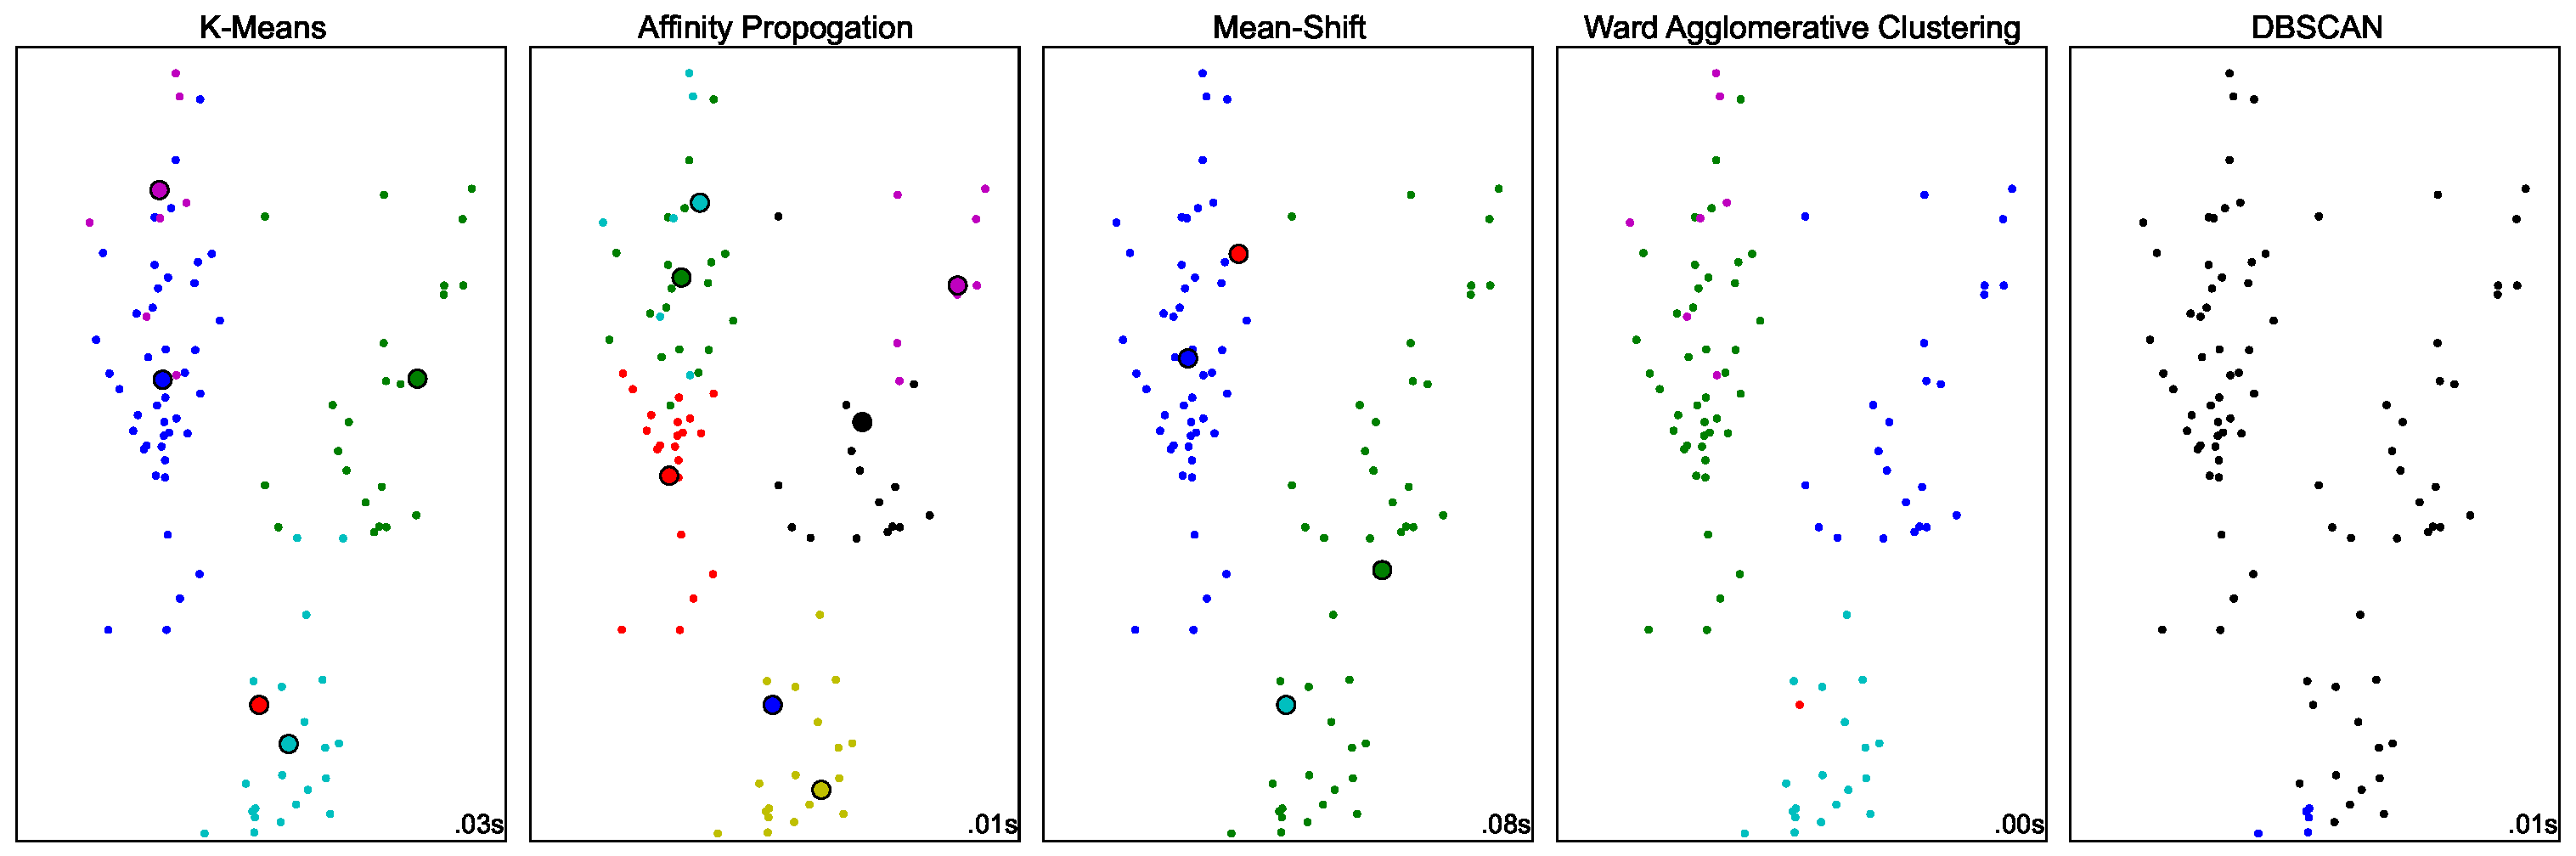
\includegraphics[width=0.8\textwidth]{clustering.eps}
    \caption{Clusters Found by the Clustering Algorithms}
    \label{fig:clusters}
\end{figure*}

After collecting all these features, we transform them to a metric space and
normalize them and generate a feature matrix and a label matrix. This is 
used by the classification algorithms that we describe in the next section.

\section{Evaluation Plan} \label{sec:eval}

\section{Classification} \label{sec:classfication}

Clustering was our first approach as an unsupervised algorithm seemed
to best fit the data at hand. As such, we tried the following methods,
all of which are inbuilt in scikit-learn:\\

\begin{itemize}
\item K-Means
\item Affinity Propagation
\item Mean-Shift
\item Ward Agglomerative Clustering
\item DBSCAN
\end{itemize}

\begin{figure*}[h!]
    \centering
    \fbox{\includegraphics[width=\linewidth]{figure/tree_4.pdf}}
    \caption{Decision tree with max depth set to 4.}
    \label{fig:tree_4}
\end{figure*}

\begin{figure*}[h!]
    \centering
    \fbox{\includegraphics[width=\linewidth]{figure/tree_7.pdf}}
    \caption{Decision tree with max depth set to 7.}
    \label{fig:tree_7}
\end{figure*}

The clusters found by each algorithm can be seen in
\cref{fig:clusters}. We also calculated common clustering metrics such
as homogeneity, completeness, and V-measure. These results can be
found in \cref{fig:clustering-metrics}. From the results, we notice
immediately that DBSCAN does not work well with our data. Indeed, it
does not find any distinct clusters at all. However, K-Means and Ward
Agglomerative Clustering algorithms perform well. 
Both of these algorithms require number of clusters as a 
parameter. 
However, this is not a restriction for our problem as we
know the number of benchmarks - and hence the number of clusters -
that we have.

In addition to evaluating clustering algorithms, we also evaluated
Support Vector Machines, a supervised classifier. While real-world
data will not be labeled and hence a supervised classifier cannot be
used, it is still useful to see how effective our features are in
discriminating between benchmarks. Using a simple two-fold
cross-validation, we found that a simple SVM with an RBF kernel
achieved 86\% precision but with a very high standard deviation of
28\%. However, this is still a very strong result as it indicates that
our features effectively separate our data into our desired
classes. 
We plan to validate the classifier on more sophisticated heterogeneous 
real-world workloads as part of our stretch goal.

The immediate next step is to build an estimator that allows us to address the
second goal of this project. We already have the infrastructure required
for collecting metrics and features required for solving this problem.
We plan to explore different machine learning algorithms to solve this
problem in the coming weeks.

\begin{figure*}[h!]
    \centering
	\subfloat[\label{fig:dt_depth}]{\includegraphics[width=0.4\linewidth]{figure/depth.pdf}}
	\subfloat[\label{fig:dt_leaves}]{\includegraphics[width=0.4\linewidth]{figure/leaves.pdf}}
	\caption{Impact of max depth and max leaf nodes on the accuracy of the
    decision tree.}
\end{figure*}

\begin{table}[h!]
\centering
\small{
  \centering
  \begin{tabular}{l|llll} 
	\toprule
   		Class &  Precision  &  Recall &  F1-score  &  Support  \\    
    \midrule
		0.0   &    1.00   &   0.00   &   1.00   &     84   \\
        1.0   &    0.99   &   1.00   &   0.99   &     74   \\
        2.0   &    0.98   &   0.99   &   0.98   &     81   \\
        3.0   &    0.54   &   0.39   &   0.45   &     18   \\
        4.0   &    1.00   &   1.00   &   1.00   &     69   \\
        5.0   &    1.00   &   0.99   &   0.99   &     70   \\
        6.0   &    1.00   &   0.95   &   0.97   &     60   \\
        7.0   &    0.41   &   0.95   &   0.57   &     19   \\
        8.0   &    0.00   &   0.00   &   0.00   &     17   \\
        9.0   &    0.56   &   0.52   &   0.54   &     27   \\
    \midrule
Avg / Total   &    0.90   &   0.91   &   0.90   &    519   \\
   \bottomrule
   \end{tabular}
 }
%\nocaptionrule
\caption{Per-class accuracy of the default decision tree.}
\label{tab:dt_stats}
\end{table}


% -----------------------------------------------
% Estimated number of clusters: 10
% Homogeneity: 0.614
% Completeness: 0.628
% V-measure: 0.621
% Adjusted Rand Index: 0.429
% Adjusted Mutual Information: 0.606
% [2 8 9 ..., 3 1 1]
% Silhouette Coefficient: 0.111
% 
% Metrics for Affinity Propogation
% -----------------------------------------------
% Estimated number of clusters: 88
% Homogeneity: 0.654
% Completeness: 0.317
% V-measure: 0.427
% Adjusted Rand Index: 0.067
% Adjusted Mutual Information: 0.248
% [72  8 22 ..., 30 74 39]
% Silhouette Coefficient: 0.082
% 
% Metrics for Mean-Shift
% -----------------------------------------------
% Estimated number of clusters: 2
% Homogeneity: 0.012
% Completeness: 0.368
% V-measure: 0.024
% Adjusted Rand Index: -0.001
% Adjusted Mutual Information: 0.010
% [0 0 0 ..., 0 0 0]
% Silhouette Coefficient: 0.517
% 
% Metrics for Ward Agglomerative Clustering
% -----------------------------------------------
% Estimated number of clusters: 10
% Homogeneity: 0.589
% Completeness: 0.635
% V-measure: 0.611
% Adjusted Rand Index: 0.458
% Adjusted Mutual Information: 0.581
% [0 4 5 ..., 4 2 6]
% Silhouette Coefficient: 0.097

\section{Estimation} \label{sec:estimation}

\begin{figure*}
\centering
\subfloat[\label{fig:lasso_latency_alphas}]{\includegraphics[width=0.4\linewidth]{figure/lasso_latency_mutate.pdf}}
\subfloat[\label{fig:lasso_throughput_alphas}]{\includegraphics[width=0.4\linewidth]{figure/lasso_throughput_mutate.pdf}}

\caption{Performance of Lasso for various $\alpha$ values for (a)
  latency and (b) throughput on the Wikipedia benchmark}
\label{fig:lasso_alphas}
\end{figure*}

\begin{figure*}
\centering
\subfloat[\label{fig:gp_latency_theta0s}]{\includegraphics[width=0.4\linewidth]{figure/gp_latency_mutate.pdf}}
\subfloat[\label{fig:gp_throughput_theta0s}]{\includegraphics[width=0.4\linewidth]{figure/gp_throughput_mutate.pdf}}

\caption{Performance of Gaussian Process Regression with absolute
  exponential autocorrelation for various $\theta_0$ values for (a)
  latency and (b) throughput on the Wikipedia benchmark}
\label{fig:gp_theta0s}
\end{figure*}

\begin{table*}[h!]
  \centering
  \begin{adjustbox}{max width=\linewidth}
    \begin{tabular}{ll}
      \toprule
      Feature Name                   & Feature Meaning                                                     \\
      \midrule
      PG\_Cache\_Hits                & Number of buffer hits in this table                                 \\
      PG\_Index\_Hits                & Number of buffer hits in all indexes on this table                  \\
      PG\_Index\_scans               & Number of index scans initiated on this
      table                       \\
      PG\_rows\_inserted             & Number of rows inserted by queries in this database                 \\
      PG\_rows\_returned             & Number of rows returned by queries in this database                 \\
      PG\_rows\_updated              & Number of rows updated by queries in this database                  \\
      PG\_sequential\_scans          & Number of sequential scans initiated on this table                  \\
      PG\_transactions\_committed    & Number of transactions in this database that have been committed    \\
      PG\_transactions\_rolled\_back & Number of transactions in this database that have been rolled back  \\
      autovacuum                     & Number of times the autovacuum daemon vacuumed this table           \\
      commit\_delay                  & Time delay before a transaction attempts to flush the WAL buffer    \\
      fsync                          & Enable making sure that updates are physically written to disk      \\
      shared\_buffers                & Amount of memory the database server uses for shared memory buffers \\
      track\_activities              & Enable the collection of information on the executing commands      \\
      wal\_buffers                   & Amount of shared memory used for WAL data                           \\
      wal\_level                     & Determine how much information is written to the WAL                \\
      wal\_writer\_delay             & Specify the delay between activity rounds for the WAL writer        \\
      \bottomrule
    \end{tabular}
  \end{adjustbox}

  \caption{Some of the influential features for throughput estimation.}
  \label{tab:influential_features_for_throughput}
\end{table*}

\begin{table*}[h!]
  \centering
  \begin{adjustbox}{max width=\linewidth}
    \begin{tabular}{ll}
      \toprule
      Feature Name          & Feature Meaning                                                    \\
      \midrule
      PG\_index\_scans      & Number of index scans initiated on this table                      \\
      PG\_sequential\_scans & Number of sequential scans initiated on this table                 \\
      fsync                 & Enable making sure that updates are physically written to disk     \\
      synchronous\_commit   & Whether transaction commit will wait for WAL records to be flushed \\
      \bottomrule
    \end{tabular}
  \end{adjustbox}

  \caption{Influential features for latency estimation.}
  \label{tab:influential_features_for_latency}
\end{table*}

We estimate expected performance of the DBMS on a given database configuration
while executing each benchmark in the second part of our solution. 
In doing so, we hope to approximately estimate the performance of the target
workload using the model for the benchmark that the classifier in 
\cref{sec:classfication} maps the workload to.
As such, we train two estimators for each benchmark: one for database 
throughput and one for database latency.

\subsection{Gaussian Process Regression}
\label{sec:gp}

We chose to use Gaussian Process Regression, a supervised learning
method, for this task as it works well for estimating regressions with
no prior knowledge about distribution. It also gives a probabilistic
estimation, allowing for further insight about bounds and probability
of exceeding them. The Gaussian Process Regression models the data
with the function

\begin{equation*}
G(X) = f(X)^{\textrm{T}}\beta + Z(X)
\end{equation*}

where $f(X)^{\textrm{T}}\beta$ is a linear regression model and $Z(X)$
is a Gaussian process with zero mean. $X$ is the input, represented as
a vector of feature values.  In this model, we try to find the ``best
linear unbiased prediction'' (BLUP) of the process given the training
data. That is, we try to find the best function for
$\hat{G}(X) = G(X|\textrm{training data})$. Under the model, it can be
shown that $\hat{G}(X) = a(X)^{\textrm{T}}y$ where $a(X)$ is the
product of the weights with the feature values. From this model, we
can find the BLUP by solving the following optimization problem:

\begin{equation*}
a(X)^* = \arg \min\limits_{a(X)} \mathbb{E}[(G(X) - a(X)^T y)^2]
\end{equation*}

subject to the constraint $\mathbb{E}[G(X) - a(X)^T y] = 0$. Gaussian
Processes are amenable to kernels, although they are used as
correlations in this model. We use the absolute exponential
autocorrelation model in our experiments. This covariance model
calculates autocorrelation of a vector X as:

\begin{equation*}
  \exp\left( \sum_{i = 1}^n -\theta_0 |\Delta X_i| \right)
\end{equation*}

where $\theta_0$ is a the autocorrelation parameter and $\Delta X$ is
the component-wise distances at which the correlation should be
calculated. We experimented with various values of $\theta_0$ and
settled on $\theta_0 = 0.001$ as it exhibited the best performance, as
seen in \cref{fig:gp_theta0s}.

One way to measure the performance of a regression model is the
$\textrm{R}^2$ score defined as:

\begin{equation*}
  \textrm{R}^2 \equiv 1 - \frac{\textrm{SS}_{res}}{\textrm{SS}_{tot}}
\end{equation*}

In this definition, $\textrm{SS}_{res} = \sum_i (y_i - f_i)^2$ where
$y_i$ is the true value and $f_i$ is the predicted value. This term is
also known as the residual sum of squares. The other term in the
definition is $\textrm{SS}_{tot} = \sum_i (y_i - \bar{y})^2$ where
$y_i$ is the true value and $\bar{y}$ is the mean of all the true
values. This is proportional to the variance of the true values. From
this definition of the $\textrm{R}^2$ score, we see that the maximum
value is 1 and that it indicates that the model perfectly predicted
the observed data. A score less than 1 indicates that the model was
not perfect and a score of zero indicates that the model is no better
at predicting the values than the mean of the true
values. \cref{fig:gp_r2} shows
the median $\textrm{R}^2$ score across the estimators for all
benchmarks as a red line. The shaded green region indicates a single
standard deviation spread. We infer from the figures that we can
train a good estimator with as few as 600 samples. In
addition, the estimators become collectively better as more data is
provided, as evidenced by the shrinking green region as number of
samples increases.

One example of a highly accurate performance estimator is the latency estimator
for the Wikipedia benchmark. This estimator has a high $\textrm{R}^2$
score of 0.9734. Looking at the actual and predicted latency values in
\cref{fig:latency_wikipedia}, we find that the
predicted distribution mimics the actual one very closely, with only a
slight dip into negative latency predictions. We believe this
estimator can be even stronger if we encode constraints for possible
predictions, such as positive values only.

One example of a less accurate performance estimator is the throughput
estimator for the balanced YCSB benchmark. This estimator has a lower
$\textrm{R}^2$ score of 0.7090. Looking at the actual and predicted
throughput values in \cref{fig:throughput_ycsb_balanced}, we see that
the estimator fails to handle the holes in throughput seen in the
actual values. We believe these isolated throughput values are due to
environmental factors that are not reflected in the feature set such
as load on the machine and other processes' resource usages. A more
``global'' set of features across the whole system rather than just
pertaining to the database may help train better estimators.

\subsection{Lasso Regression}
\label{sec:lasso}

To gain more insight about what parameters affected performance the
most, we performed Lasso Regression to determine the most influential
features. Lasso regression encourages sparse coefficients in its
solution, so it is a good method for finding the most important
features for a particular problem. It works by optimizing this
objective function :

\begin{equation*}
  \min\limits_{w}
  \frac{1}{2n_{\textrm{samples}}} \|Xw - y\|_2^2 + \alpha \|w\|_1
\end{equation*}

which is a simple least squares linear regression with the lasso
constraint added under weight $\alpha$. A higher value for $\alpha$
encourages sparser solutions while a lower value relaxes this
constraint. We experimented with different values of alpha and settled
on using $\alpha = 0.001$ as it exhibited the best performance, as seen in
\cref{fig:lasso_alphas}.

 These features are summarized in
\cref{tab:influential_features_for_throughput} and
\cref{tab:influential_features_for_latency}. Confirming general
intuition, throughput seems to be greatly affected by all operation
types along with options that add delays (e.g. bgwriter\_delay,
commit\_delay) or constrain how relaxed the database can be about
transaction execution (e.g. fsync, synchronous\_commit). It
is, however, very interesting to note that latency seems 
primarily affected only by operations that take a long time to 
complete and not the type of operations or hard delays introduced into the
system.

In a practical implementation of our estimator, we will not be able
to collect performance statistics while estimating performance for
a specific configuration as we do not actually execute the workload
in that configuraion. So, we eliminated the features pertaining to 
throughput and latency from consideration while estimating 
performance metrics.
However, these features are available in the training dataset. 
We believe that we can use graphical models to infer these 
missing throughput and performance features in the test data 
before estimation. We plan to explore this technique in 
future work.
\section{Conclusion} \label{sec:conclusion}

DBMS performance tuning is a niche skill that requires much experience
and experimentation to get correct. However, machine learning
techniques can help automate this process by using prior knowledge to
estimate performance without having to go through a time-consuming
experiment. To achieve this goal, we have taken a two-step approach
where we first use map a workload to a well-studied benchmark. Armed with
this information, we then use a regression estimator to estimate the
performance of the benchmark under a given environment.

Using decision trees to map the workloads, we find that we can
classify workloads using a few defining characteristics. The decision
trees produces effectively discriminate between the different
benchmarks and are very intuitive. For performance estimation, we trained estimators
using Gaussian Process Regression that show very accurate estimation
of database throughput and latency. In addition, these highly accurate
estimators can be trained with as few as 600 samples! Further analysis
of performance estimation using Lasso Regression provided key insights
into the features that are most influential in determining throughput
and latency.

While promising, this work only uses synthetic data generated from
OLTPBench. We hope to continue this work using a larger dataset that
includes mixtures of benchmarks along with real-world workloads. In
addition, we hope to extend our data to include performance
estimation across different hardware profiles and DBMS's. This larger
amount of more realistic data should help us get additional insights
about how best to estimate performance of arbitrary database workloads.

\clearpage
\balance

\bibliographystyle{plain}
\bibliography{ref}

\end{document}
% end doc
